%%%%%%%%%%%%%%%%%%%%%%%%%%%%%%%%%%%%%%%%
% Class options                        %
%%%%%%%%%%%%%%%%%%%%%%%%%%%%%%%%%%%%%%%%
% Orientation:                         %
% portrait (default), landscape        %
%                                      %
% Paper size:                          %
% a0paper (default), a1paper, a2paper, %
% a3paper, a4paper, a5paper, a6paper   %
%                                      %
% Language:                            %
% english (default), norsk             %
%%%%%%%%%%%%%%%%%%%%%%%%%%%%%%%%%%%%%%%%
\documentclass{../psuposter}
\renewcommand{\templateimagepath}{../} 

\usepackage{lipsum}                                % Dummy text
%\usepackage[figwidth = 0.98\linewidth]{todonotes}  % Dummy image (and more!)
\usepackage[absolute, overlay]{textpos}            % Figure placement
%\usepackage{hyperref}
\setlength{\TPHorizModule}{\paperwidth}
\setlength{\TPVertModule}{\paperheight}

\setcitestyle{numbers,square}


\title{Modeling the strong-field dynamics of binary neutron star merger}
\author{Sebastiano Bernuzzi \inst{1}}
%% Optional:
\institute
{
    \inst{1} Friedrich-Schiller University, Institute for Theoretical Physics
}
% Or:
%\institute{Contact information}


%% Remove footline:
%\setbeamertemplate{footline}{}


\begin{document}
\begin{frame}
\begin{columns}[onlytextwidth]


\begin{column}{0.45\textwidth - 1cm}
    \begin{block}{Speaker Biographic Summary}
    	\begin{center}
    		
\includegraphics[width=0.6\textwidth]{images/sebastiano-bernuzzi}
    	\end{center}
    	\href{https://www.tpi.uni-jena.de/~bernuzzi/about.html}{Sebastiano Bernuzzi} is a theorist, based at the Institute for Theoretical Physics at Friedrich-Schiller University Jena, with a strong background  in numerical relativity. After completing his PhD at Parma University, Sebastiano held postdoc positions at Jena University and Caltech. He was honored as a Rita Levi Montalcini fellow while an assistant Professor at Parma University, and is presently a European Research Council Starting Grant fellow. \cite{Bernuzzi}  
    \end{block}

    \begin{block}{Research Interests}
        Sebastiano's research focuses on modeling the dynamics of compact object mergers using numerical techniques in general relativity. He has developed computational methods for studying gravitational waves and their electromagnetic counterparts using the largest supercomputers in the world. Sebastiano also works with the LIGO and Virgo scientific collaboration to support gravitational-wave astronomy observations. 
        \begin{center}
	    	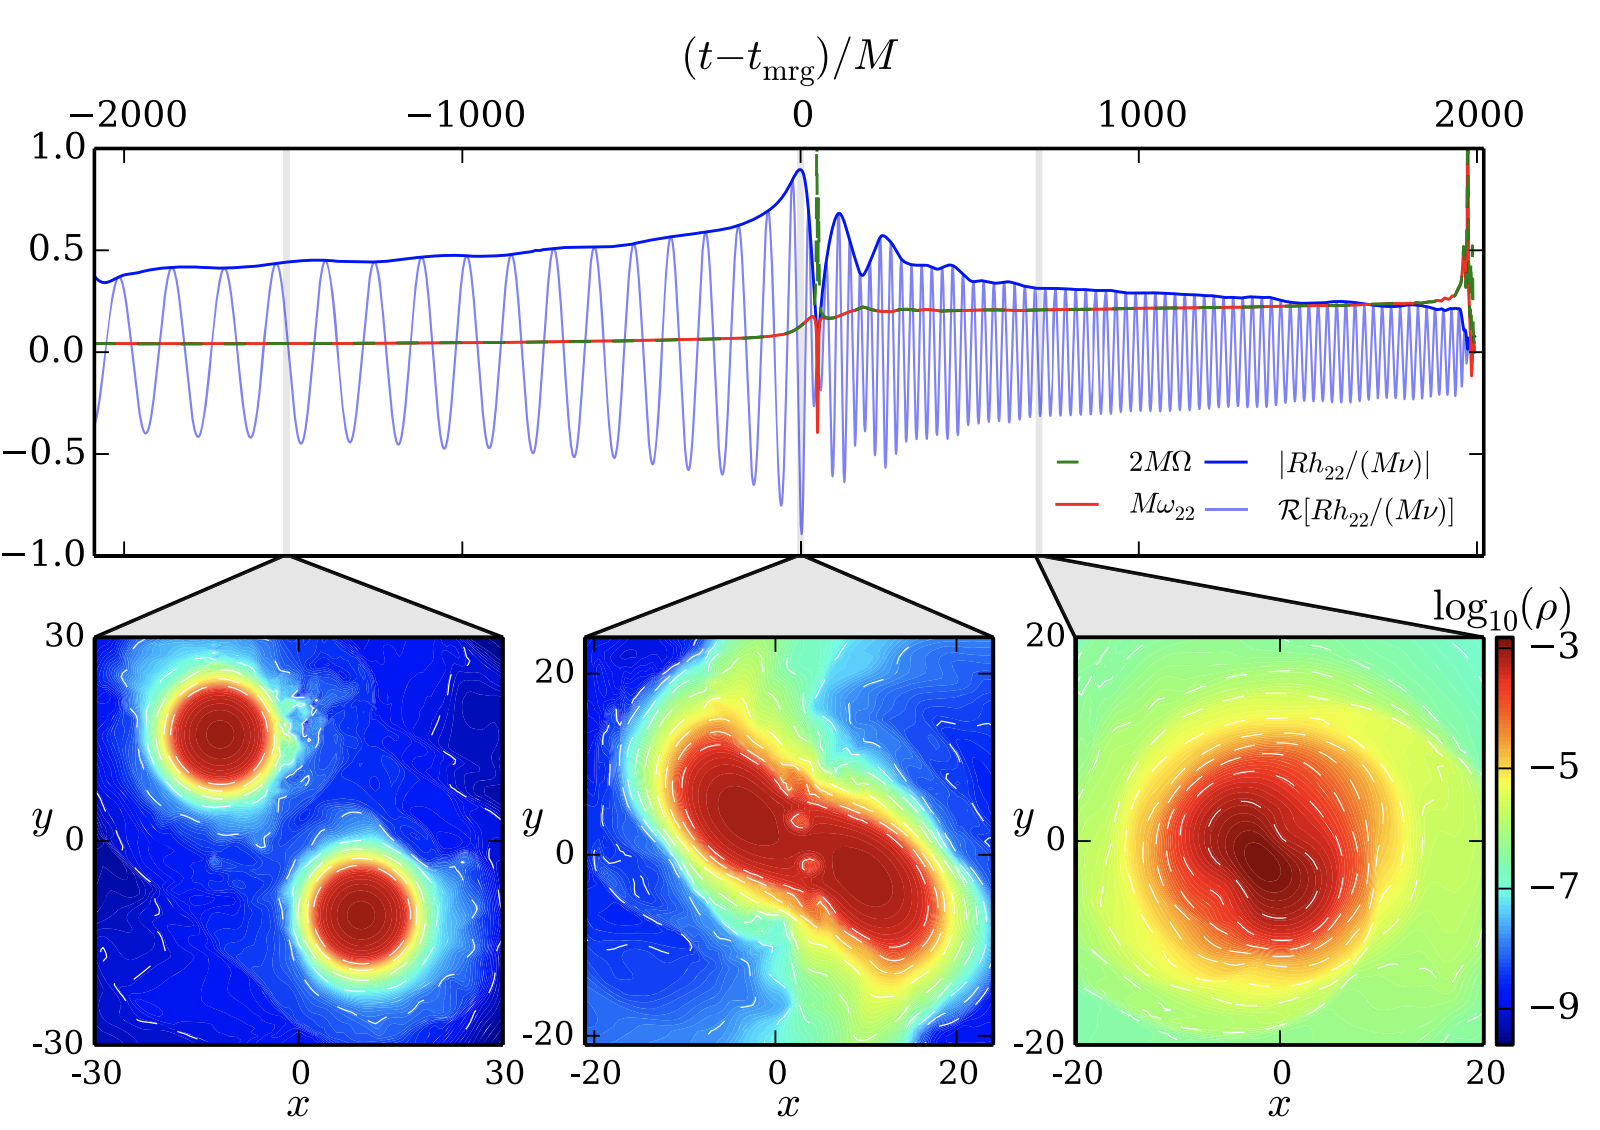
\includegraphics[width=0.98\textwidth]{images/bernuzzi-merger}    		
    	\end{center}
    	\textit{Above: simulated binary neutron star merger waveform}. \cite{bernuzziModelingCompleteGravitational2015}
    \end{block}
\end{column}


\begin{column}{0.55\textwidth - 1cm}
    \begin{block}{Talk Abstract}
        The observation of gravitational and electromagnetic waves from a binary neutron star merger in August 2017 conveyed key information on the nature of matter at supranuclear densities, on the origin of short-gamma ray burst, on the production site of of heavy elements via r-process nucleosynthesis, and on cosmography. Future multimessenger observations of this kind hold the promise to convey unprecedent insights on some of the most fundamental physics questions. A crucial and necessary ingredient to intepret these observations is the precise knowledge of the dynamics of the sources. I will talk about recent developments on the modeling of neutron star mergers using numerical simulations in general relativity. I will focus on the exploration of the the merger remnant and mass ejecta, and the dependence of the merger outcome on the binary parameters. I will discuss detailed models of the gravitational signal for the complete (inspiral-merger-postmerger) gravitational spectrum.
    \end{block}

    \begin{block}{Brief Background}
        Binary neutron star (BNS) mergers produce a compact central object surrounded by an accretion disk (depicted below). If the remnant does not quickly collapse into a black hole (BH), then its early evolution is dominated by gravitational wave emission. After this dynamical phase, the long-term evolution is determined by energy and angular momentum evolution due to magnetohydrodynamics (MHD) and weak interactions in the fluid.
        \cite{bernuzziNeutronStarMerger2020}
        \begin{center}
	    	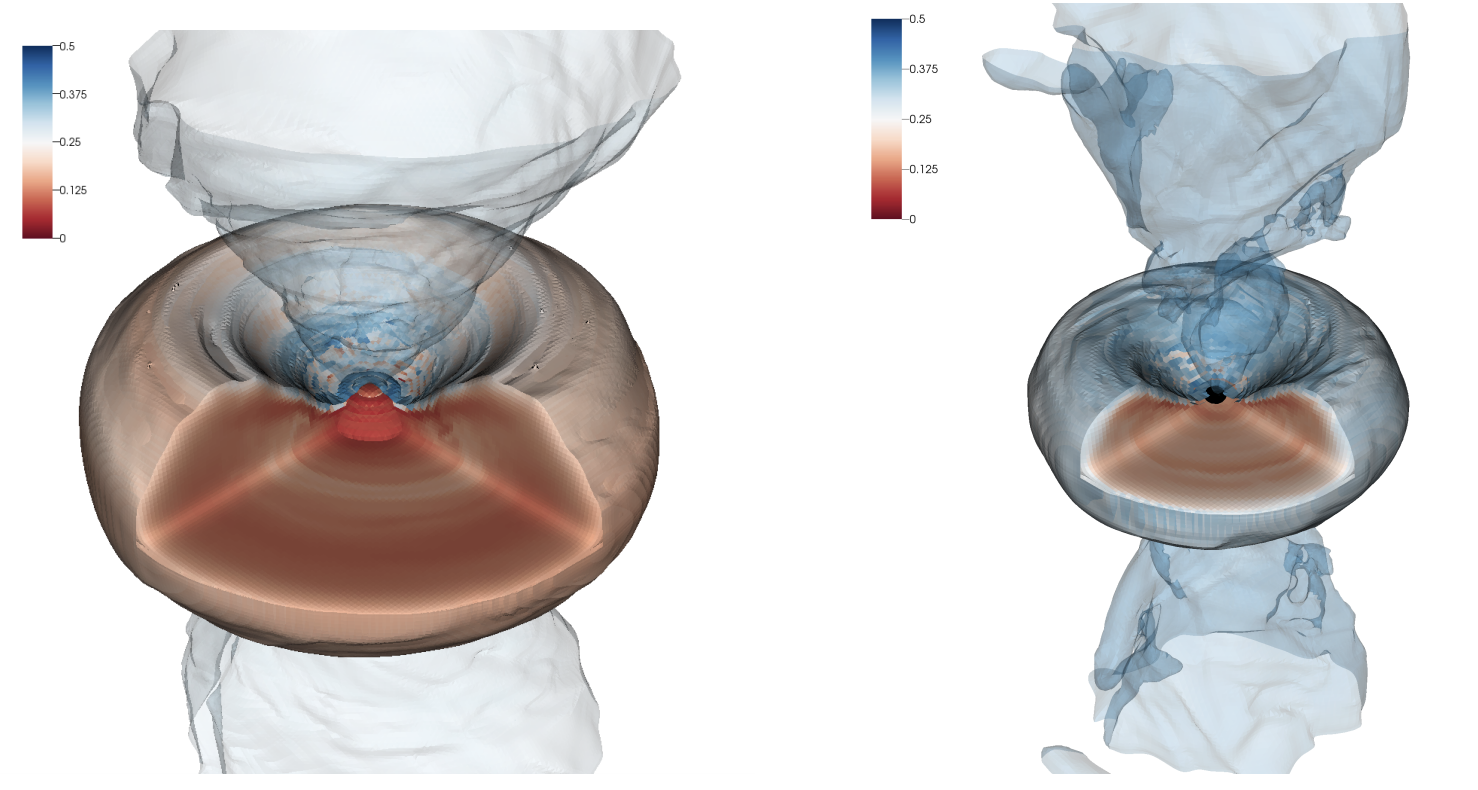
\includegraphics[width=0.6\textwidth]{images/bernuzzi-remnant}    		
    	\end{center}
%        $$\lambda_1 \tilde{\lambda}_1 + \lambda_2 \tilde{\lambda}_2 + \lambda_3 \tilde{\lambda}_3 = 0 \iff \left\{ \begin{split}
%        		(A): & \lambda_1 \propto \lambda_2 \propto \lambda_3 \\
%        		(B): & \tilde{\lambda}_1 \propto \tilde{\lambda}_2 \propto \tilde{\lambda}_3 \\
%	        \end{split} \right\}$$
%        \lipsum[3]
		Inspiral dynamics for BNS differ from BH due to tidal interactions between the NSs. The distortion of the mass distribution due to these tidal effects is measured by the Love numbers $k_l^A$. These can be used to define a tidal coupling constant $\kappa_2^T$, which specifies the tidal interactions in the binary to leading Newtonian order. While the details can only be determined by simulation, these quantites are essential for characterizing the output data. It is also possible to characterize results in a gauge invariant way, using the reduced binding energy $E_b$ and the angular momentum of the binary $j$.
        \cite{bernuzziNeutronStarMerger2020}
    \end{block}

    \begin{block}{References}
%        \lipsum[1]
        \bibliographystyle{aipnum4-1}
		\bibliography{../references}
    \end{block}

%    \begin{block}{Contact information}
%        \lipsum[75]
%    \end{block}
\end{column}


\end{columns}


\begin{textblock}{0.5}(0.18, 0.94)
    \color{white}
    \sffamily
    \textbf{Eberly College of Science}
    \\
    Department of Physics
    
\end{textblock}


\end{frame}
\end{document}